\documentclass[11pt]{exam}
\usepackage{listings}
\usepackage{pdfsync}

%
%  Created by Brad Miller on 2005-05-13.
%  Copyright (c) 2005 Luther College. All rights reserved.
%
%

\newif\ifpdf
\ifx\pdfoutput\undefined
\pdffalse % we are not running PDFLaTeX
\else
\pdfoutput=1 % we are running PDFLaTeX
\pdftrue
\fi

\ifpdf
\usepackage{subfigure}
\usepackage[pdftex]{graphicx}
\else
\usepackage{graphicx}
\fi

%
%  Update these values for running headers
%
\firstpageheader{\bf\Large CS-151}{\bf\Large Final Exam}{\bf\Large
  May 16, 2005 }
\runningheader{CS 151}{}{Final Exam}
\addpoints

\begin{document}

\begin{center} 
  \fbox{\fbox{\parbox{5.5in}{\centering This Exam is being given under
        the guidelines of the \textbf{Honor Code}. You are expected to
        respect those guidelines and to report those who do not.
        Answer the questions in the spaces provided. If you run out of
        room for an answer, continue on the back of the page.  There are
      \numquestions\  questions for a total of  \numpoints\ points.}}}
\end{center} 

% setup standard options for the including code fragments
\lstset{language=Python,numbers=left}

\vspace{0.1in} 
\hbox to \textwidth{Name:\enspace\hrulefill} 

% Questions start here:
\begin{questions}

\question Given the following list of numbers \lstinline{x = [13, 24, 5, 7, 9, 17, 32, 27, 2]}

\begin{parts}
\part[10]  Create a binary search tree and insert each of the numbers.  Show the final tree.
\vspace{3in}
\part[10]  Create a binary heap and insert the numbers one at a time into the heap. Show both the tree and list representation of the heap after all the numbers are inserted.
\vspace{3in}
\end{parts}

\newpage
\question Given the binary tree shown below:
\begin{figure}[h!]
    \begin{center}
        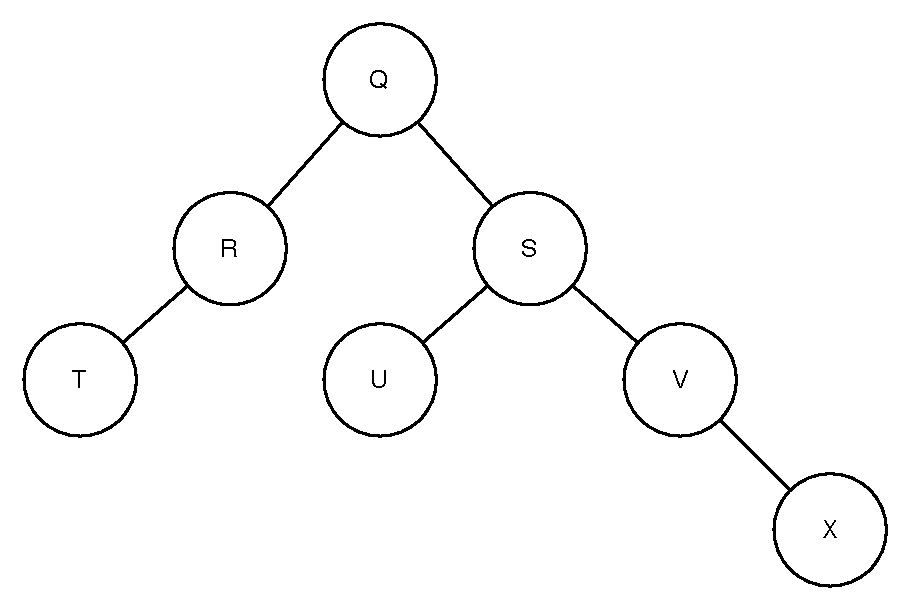
\includegraphics[height=3in]{binaryTree}
    \end{center}
\end{figure}
\begin{parts}
    \part[5] Perform a pre-order traversal of the tree.  Write out the name of each node in the order it is visited.
    \vspace{1in}
    \part[5] Perform a post-order traversal of the tree. Write out the name of each node in the order it is visited. 
    \vspace{1in}
\end{parts}

\newpage
\question
Yertlenet is a primitive form of networking that was used at Luther college up until the mid 1980's.  Yertlenet uses turtles as a message transport mechanism and requires that special one-way channels be dug between the buildings on campus to facilitate turtle navigation. A Messages is routed from building $x$ to building $y$ by placing a message on the back of a turtle and setting the turtle in the channel leading to the next building.  To facilitate routing, each building employed a student worker to receive incoming messages and if necessary move the turtle to the channel leading to the next building.  

You have just been hired as the new student worker for building one. Being a CS major you decide that you want to be the best turtle router on campus and therefore will create a graph of Yertlenet and figure out the optimum routing for messages that come through your building. The following table shows the information describing the Yertlenet connections column one is the start building, column two is the end building, and column three is the cost of the link.

\begin{verbatim}
1 2 10
1 3 15
1 6 5
2 3 7
3 4 7
3 6 10
4 5 7
6 4 5
5 6 13
\end{verbatim}

\begin{parts}
\part[10]
Draw the directed graph represented by the above table.
\vspace{8in}
\part[10]
Using Dijkstras algorithm, find the shortest path to each other building on campus.  Make sure that you show the intermediate steps as you run the algorithm.
\vspace{6in}
\part[5] Show the table that you will use to decide which channel to put the turtle in to send a message to each building on campus.
\vspace{1.5in}
\end{parts}

\newpage
\question[10]  Recall that the height of the tree is defined as the number of edges between the root and the deepest leaf in the tree.  Write a function height(t) that takes a tree as a parameter and returns the height of the tree.  \textit{Hint 1} The methods for a tree are as follows:
\begin{itemize}

	\item BinaryTree()  Create a new instance of a binary tree.
    \item getLeftChild() Return the binary tree corresponding to the left child of the current node.
    \item getRightChild() Return the binary tree corresponding to the right child of the current node.
    \item setRootVal(x) Store the object in parameter x in the current node.
    \item getRootVal() Return the object stored in the current node.
    \item insertLeft(x) Create a new binary tree and install it as the left child of the current node.
    \item insertRight(x) Create a new binary tree and install it as the right child of the current node.

\end{itemize}

\textit{Hint 2} The height function is easy if you think recursively.

\newpage
\question  Consider the following classic problem:  You have two jugs a 4-gallon and a 3-gallon. Neither of the jugs have markings on them. There is a pump that can be used to fill the jugs with water. You can pour water from one jug to another, and you can empty a jug on the ground.  Note when you pour water from one jug to another you are can either pour all the water from the first into the second, or you can pour the water from the first to the second until the second is full.  How can you get exactly get two gallons of water in the 4 gallon jug?

\begin{parts}
    \part[10]  How would you represent this problem as a graph?
    \vspace{8in}
    
    \part[10]  Apply the Breadth First Search algorithm to this problem.  
\end{parts}

\end{questions}

\end{document}

